\section{Basics about C Programming}
\label{sec:basics}
\begin{frame}<beamer>
    \frametitle{Outline}
    \tableofcontents[currentsection]
\end{frame}

\begin{frame}
	\frametitle{Brief History about C}
	\vspace{-0.1in}
\begin{figure}
	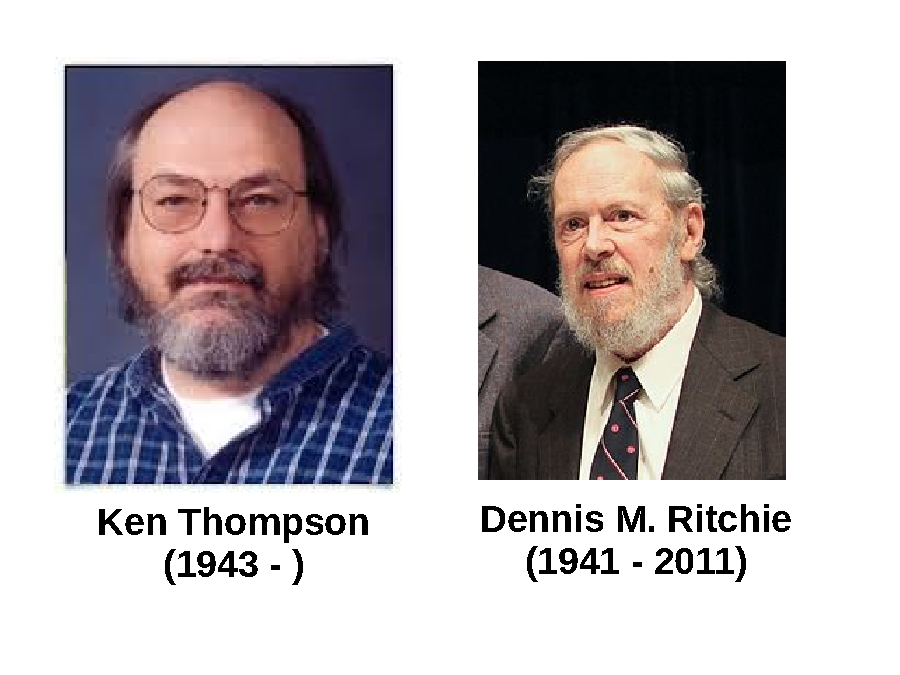
\includegraphics[width=0.5\linewidth]{figs/cuunix.pdf}
\end{figure}
\begin{itemize}
	\item {C is born in AT\&T Bell Labs along with UNIX}
	\item {The developer Dennis Ritchie and Ken Thompson were awarded with Turing Award}
	\item {C is simple:), versatile and highly efficient (70\% of assembly language efficiency)}
	\item {UNIX is one of the most stable operating systems so far developed}
\end{itemize}
\end{frame}

\begin{frame}[fragile]
	\frametitle{Your first program in C (1)}
\begin{lstlisting}[language=c]
#include <stdio.h>
int main()
{  /*start of a block*/
    printf("Hello world!\n"); /*call function 'printf'*/
    return 0;                 /*return '0' back*/
} /*end of a block*/
\end{lstlisting}
\vspace{-0.15in}
\begin{itemize}
		\item {``\#include $<$stdio.h$>$'' states that we want to use \textcolor{red}{function} defined in ``stdio.h'' }
		\item {Our code is encapsulated in a function called ``\textbf{main()}''}
		\item {In the main bordy of the function}
		\item {We output ``Hello world!'' to the screen}
		\item {``\textcolor{red}{printf()}'' is a function \textcolor{red}{defined} in ``stdio.h''}
		\item {\textcolor{blue}{include}, \textcolor{blue}{int} and \textcolor{blue}{return} are reserved keywords}
	\end{itemize}

\end{frame}


\begin{frame}[fragile]
	\frametitle{Your first program in C (2)}
\begin{lstlisting}[language=c]
#include <stdio.h>
int main()
{  
    printf("Hello world 1!\n"); 
    printf("Hello world 2!\n"); 
    printf("Hello world 3!\n"); 
    return 0;                 
} 
\end{lstlisting}
[Output]
\begin{lstlisting}[language=c]
   Hello world 1!
   Hello world 2!
   Hello world 3!           
\end{lstlisting}
\vspace{-0.15in}
\begin{itemize}
		\item {Codes are executed \textcolor{red}{from top to bottom}}
\end{itemize}

\end{frame}

\begin{frame}
	\frametitle{Popularity of C in recent decade}
	\vspace{-0.1in}
	\begin{figure}
		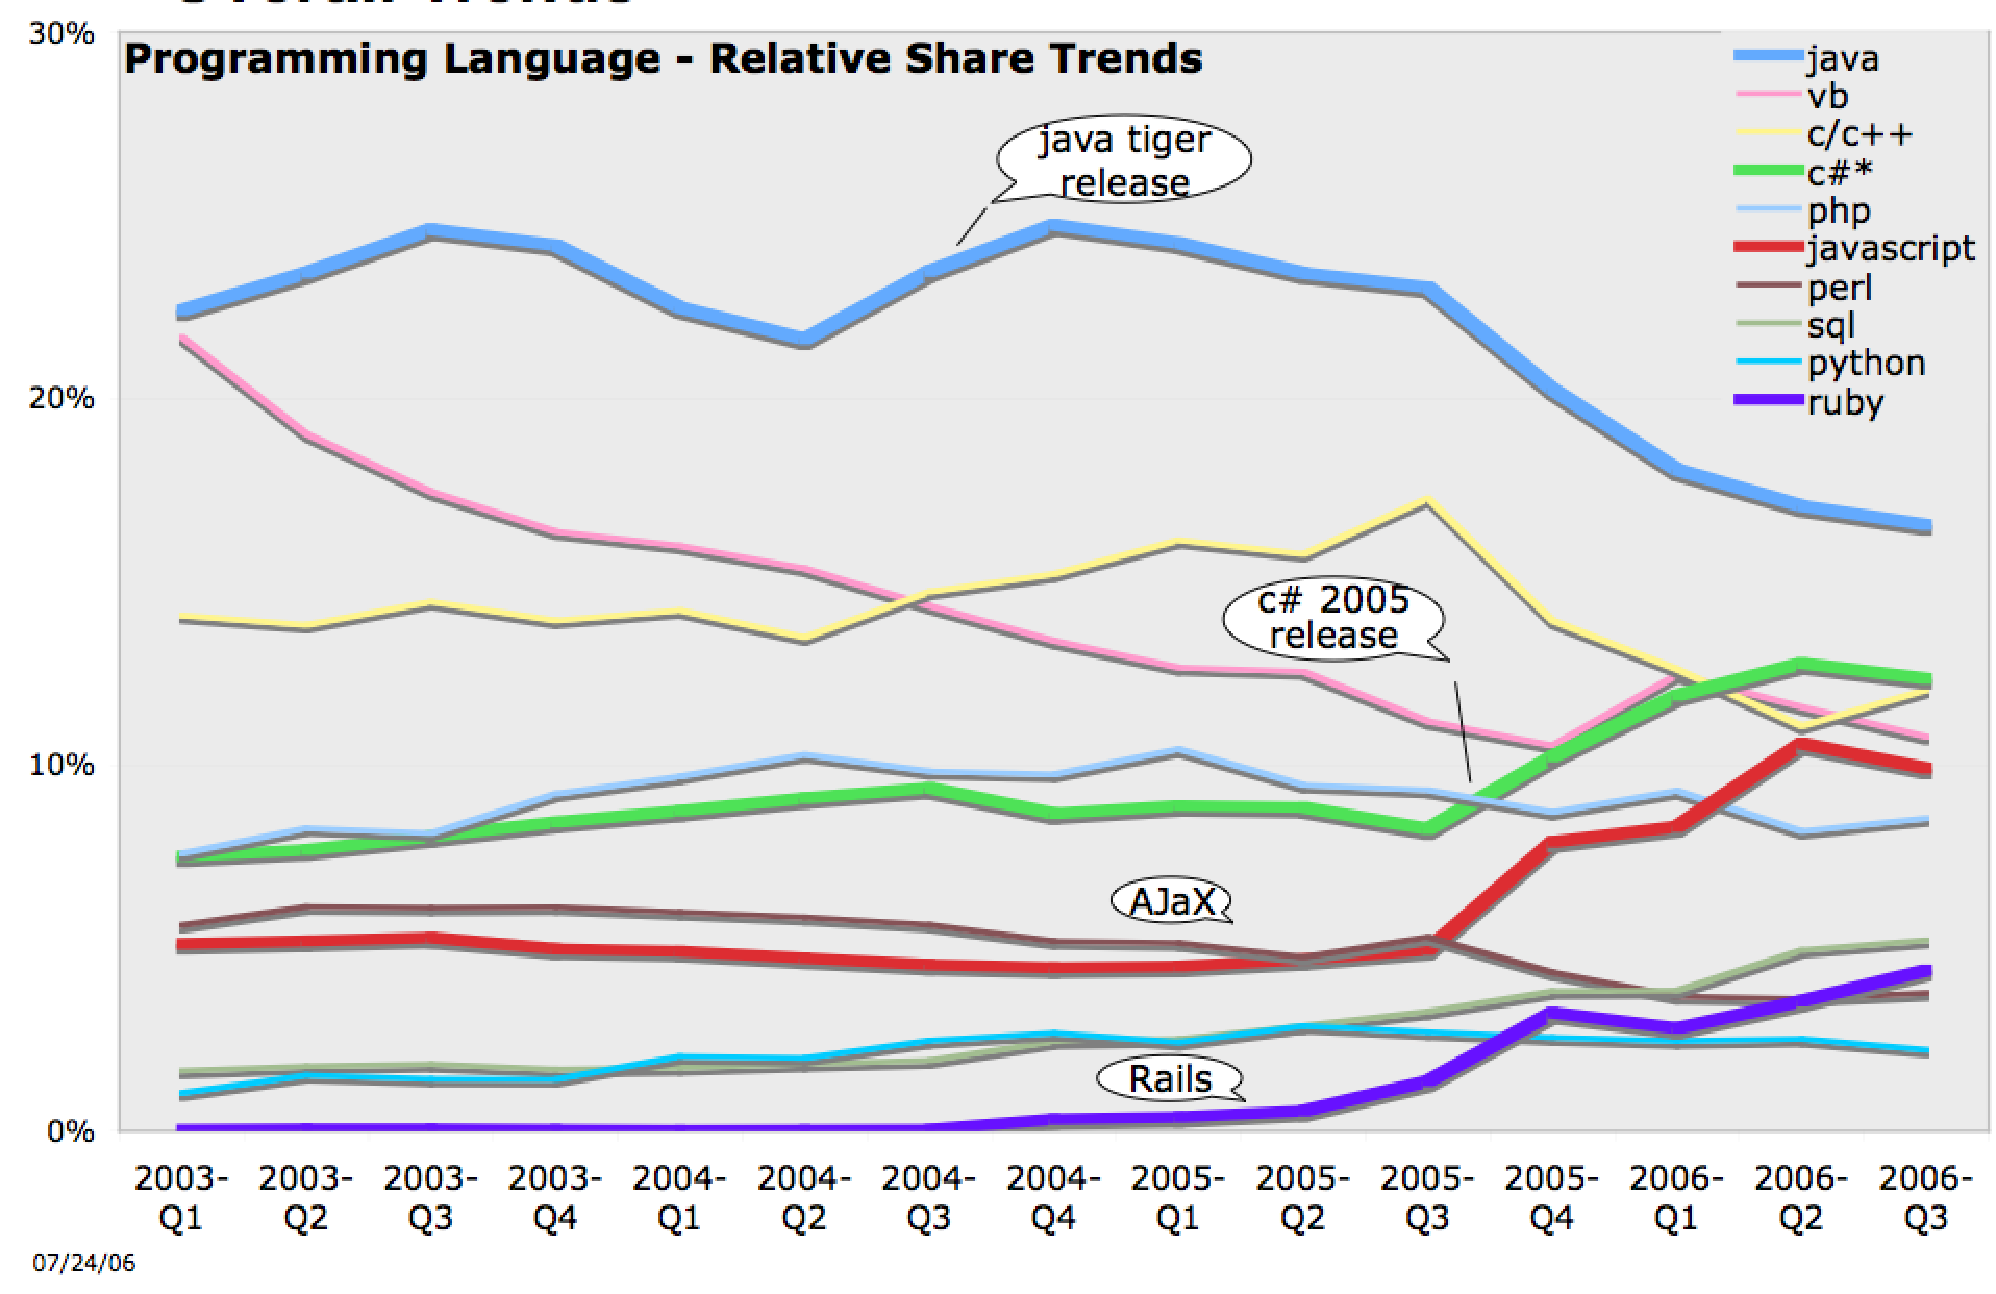
\includegraphics[width=0.85\linewidth]{figs/lang_distr.pdf}
	\end{figure}
\end{frame}


\begin{frame}
	\frametitle{Popularity of C in recent decade}
	\vspace{-0.1in}
	\begin{figure}
		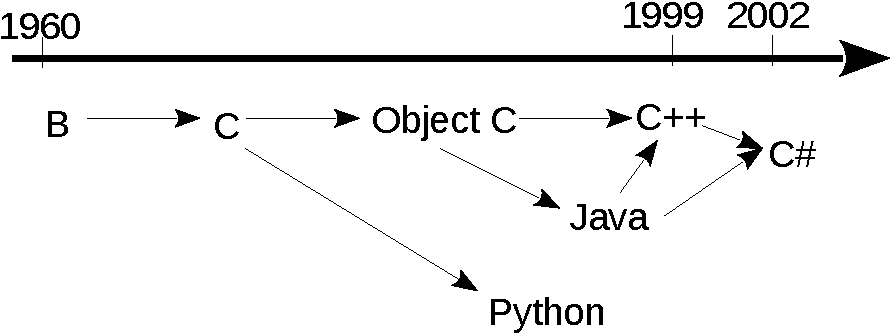
\includegraphics[width=0.85\linewidth]{figs/lag_evov.pdf}
	\end{figure}
\end{frame}


